\documentclass{primus}
\usepackage{graphicx}
\usepackage{float}
\usepackage{url}

\renewcommand{\baselinestretch}{1.3}

\title{From Exam to Education: The Math Exam/Educational Resources wiki
}

\keywords{educational learning resource, exam database, MediaWiki, online learning, wiki}

\markboth{}{From Exam to Education: The MER wiki}

\begin{document}
%\makePtitlepage
\makePtitle

\begin{abstract}
The Math Educational Resources (MER) wiki is an open online learning resource hosted at The University of British Columbia (UBC), aimed at providing math education resources for students and instructors at UBC.  In this paper, we will discuss the motivation for creating this resource on the MediaWiki platform, key features of our implementation that support student learning (including the evolution of the MER wiki from an exam database to more general learning resource), data on student use and response, potential for future development, and a brief description of how the project was implemented.
\end{abstract}

\listkeywords

\section{INTRODUCTION}\label{sec:Introduction}

The Math Exam/Educational Resources (MER) wiki is a digital collection of material aimed at improving undergraduate students’ knowledge of mathematics with a focus on first year courses at The University of British Columbia (UBC). The project, which is  maintained primarily by graduate student volunteers in the math department at UBC, began as a database of examination solutions in February 2012, and since then has evolved into an extensive library of tools that students can use to study mathematics.  These tools include access to detailed and peer-reviewed hints and solutions, focused topics pages that help navigate the database for specific types of problems and also feature short video lectures. Further, students can assign a difficulty scale to the problems they attempt and see the average rating of their peers, and embedded syllabi allow students to quickly find the relevant content for their midterm and final exams. Through thousands of students accessing the resource, we have collected a substantial amount of data on exam and course usage, as well as time periods of high traffic. This data can be used to gauge exam difficulty, to identify the amount of time and how students are spending their time studying, and to further develop the wiki to increase its effectiveness in facilitating students’ self-directed online learning.
\\\\
\noindent{}In this paper we discuss the background and implementation of the MER wiki and the particular features that contribute to its effectiveness and popularity as a learning resource.  We conclude by showing some usage statistics and user testimonials and discuss the potential future directions of the project.

\section{HISTORY AND RATIONALE}\label{sec:History_and_Rationale}
In the mid 1980s and early 1990s  a research movement studying the effects of worked examples was developed to examine the effects of this technique on learning. It was shown in \cite{CS1}, \cite{CS2}, \cite{PM} that, in general, worked examples will save students time while studying and will improve test scores on both similar problems and on problems that are more advanced than the given worked example problems themselves. Thus, it can be helpful to offer students worked solutions to previous exams as a study aid. This has been the case in the Mathematics Departments of UBC for many years.
\\\\  
\noindent{}Traditionally, the mathematics department at UBC makes its exams publically available for students shortly after they are written, albeit without solutions.  Independently from the mathematics department, solutions to these exams were sold in paper copies to undergraduate students.  As technology improved, the department started uploading their tests to the public department website, but the medium of solution delivery was essentially unchanged.  By the static nature of the product, solution packages quickly fell out of date and were arduous to update efficiently, were often riddled with typos and mathematical errors, and maintained a very poor quality control standard.  In February 2012, a group of graduate students, disatissfied with the aforementioned issues, concluded that most of the problems stemmed from the dissemination model and began researching alternative approaches.
\\\\  
\noindent{}While dissatisfaction was growing within the graduate students regarding the exam solution delivery system, UBC was independently developing a campus-wide MediaWiki\footnote{\label{ft:analytics} See \url{http://www.google.ca/analytics/}} that could collectively host a variety of university initiatives and educational products.  The format is probably best known for its use in Wikipedia.org, though it is a widespread online platform, used because of its intuitive structure and its ease of collaborative use.  Some graduate student instructors in the math department had already used the UBC wiki as an effective alternative to a traditional course webpage, in particular, because of its ease in adding and editing mathematical content and formulas.  Furthermore, this platform features an integrated version control which allows for the recovery of previous content if desired. These attributes were just a few of the reasons why a MediaWiki server emerged as the best option for the new dissemination model and using this technology, we created the MER wiki.
\\\\
\noindent{}One of the greatest features of the wiki is that it offers free and worldwide access, contrasting the model where hard-copy solutions were only sold on campus and only during specific times.  In addition, even with the open access feature, the MediaWiki system allows us to limit editing rights to mathematics experts (primarily UBC math graduate students), so that the quality of the resource can be rigorously maintained.  The main tool we use to maintain this quality is a peer-review flagging system, a tiered layer involving various reviews and revisions to content.  Students can interact with editors and each other via discussion pages and recommend changes to the content using feedback forms.  The dynamic editing process means solutions that were static and hence difficult to modify can now be easily updated to improve student understanding.  This process allows the MER wiki to improve on the limitations with the aforementioned paper-based solution packages.
\\\\
\noindent{}When this project was started in February 2012, the development team focused on setting up its basic infrastructure and adding content for various first and second year undergraduate math courses at UBC\footnote{For a brief technical survey of our implementation, please see Appendix \ref{sec:Appendix}.
}.   Even in this initial phase, there were immediate positive changes compared to the paper model.  This new model was instantaneously wider in scope and power because the content was made more widely accessible and easier to improve.  Moreover, the MER wiki featured not only solutions, but also hints and study tips, a service not available in the previous exam solution packages.  These hints offered help to students wanting to complete an independent solution before looking at the answer.  The impact of this small change to the product was significant. For the first time, the idea of simply offering solutions to students enrolled in undergraduate math classes shifted toward an enhanced learning resource.  
This notion - that the MER wiki was not simply providing solutions, but also resources and guidance for students learning mathematics - became the motivation and philosophy behind the entire project, and led to the current version of the site.  The contributors began to design solutions that instructed students on how to solve problems rather than just providing the final answer, while also explaining the mathematical concepts behind the questions.  We also introduced a tagging system that presents the questions grouped by topic, so students can review specific concepts and access relevant problems that might even come from different courses.  To better reflect the modern philosophy of the resource, we recently transitioned the identity of the wiki from Math Exam Resources to the current name, Math Exam/Educational Resources.
\\\\
\noindent{}At the time of writing, this project has over 1200 worked solutions spanning 16 courses and has been accessed over 1,000,000 times collectively for a total of over 35,000 hours collectively spent on the wiki in the first two years.  As the project has matured, we have shifted our focus to developing the online resource as an educational product.

\section{INNOVATIVE FEATURES}\label{sec:Innovative_Features}
The MER wiki came into being as an improved alternative to a paper based dissemination model.  In this section we detail key features of our implementation that make it a superior model of content dissemination and student learning.  
\\\\
\noindent{}In what follows, we define wiki contributors as those who edit wiki content, typically graduate students in the math department, and users as the people who use the content in the wiki to improve their mathematical understanding, typically undergraduate students.  

\subsection{DESIGN AND DESIGN INTENTION}\label{sec:Design_and_Design_Intention}
Our understanding, as evidenced by student use of the wiki and usage surveys is that students are seeking practice questions to solidify their problem-solving and computational skills.  They can access questions by topic to review particular question types, or by course to simulate an exam situation. For each question, the hint(s) and solution(s) are initially hidden when the page is opened.  This is designed to motivate the student into solving the questions themselves before checking solutions.  Each question page displays general problem solving advice (see Figure \ref{fig:question_page}), encouraging the student to try the question on their own, reveal the hint(s) if necessary, and finally reveal the solution(s) only when the problem is solved or if they are genuinely stuck.
\\\\
\noindent{}Once students have attempted a problem or have difficulties on how to approach the problem, they have the option to reveal hints to help with their problem solving strategy. Sometimes multiple hints are available, for example, when there is more than one natural ways to solve a problem, or when a solution warrants many steps. A user can reveal the solution at the bottom of the page and check over their work, ideally after attempting the problem for themselves.  
At the end of each question, students have a chance to rate the question’s difficulty and/or give us feedback (see sections \ref{sec:Rating_Bar} and \ref{sec:Student_Feedback}).  Below, one can see a sample of this process.
\begin{figure}[H]
\centering
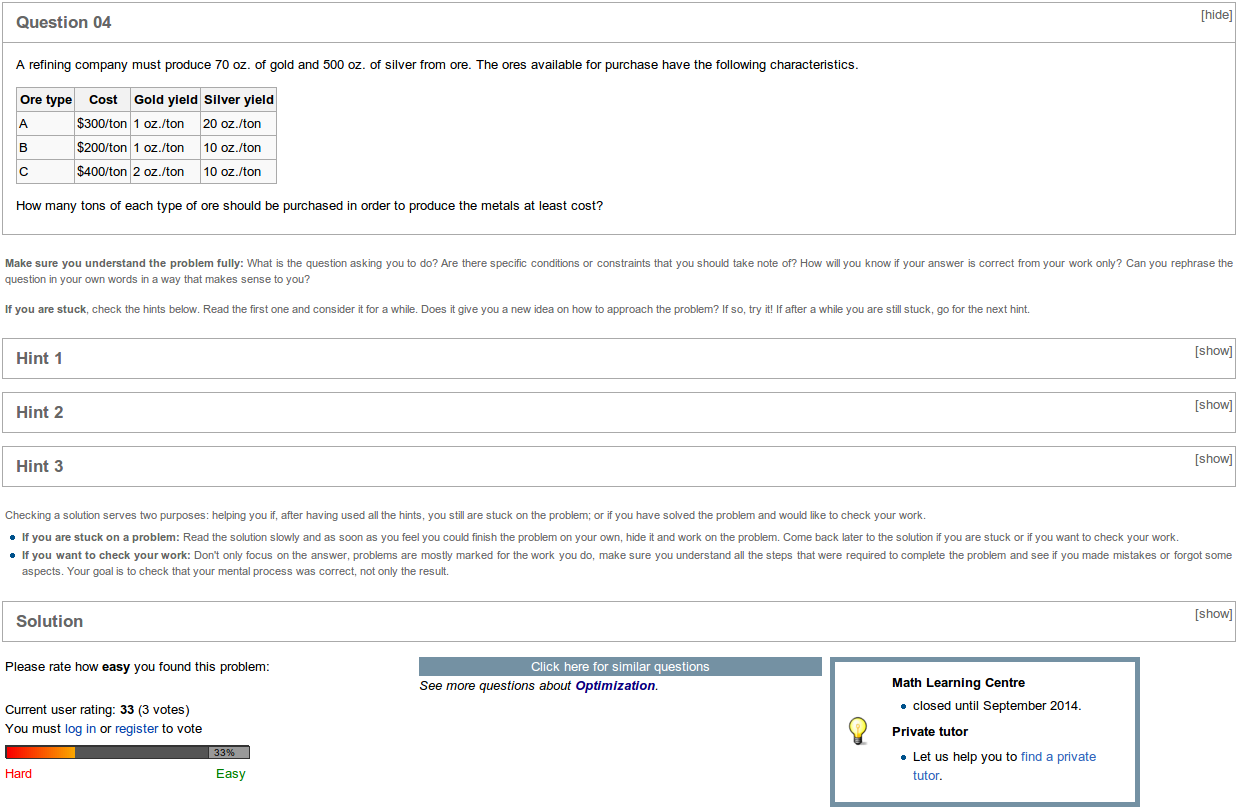
\includegraphics[width=\textwidth]{figs/Question_Page.png}
\caption{A representative example of what a student sees when they click on one of the questions in the MER wiki.}\label{fig:question_page}
\end{figure}
\begin{figure}[H]
\centering
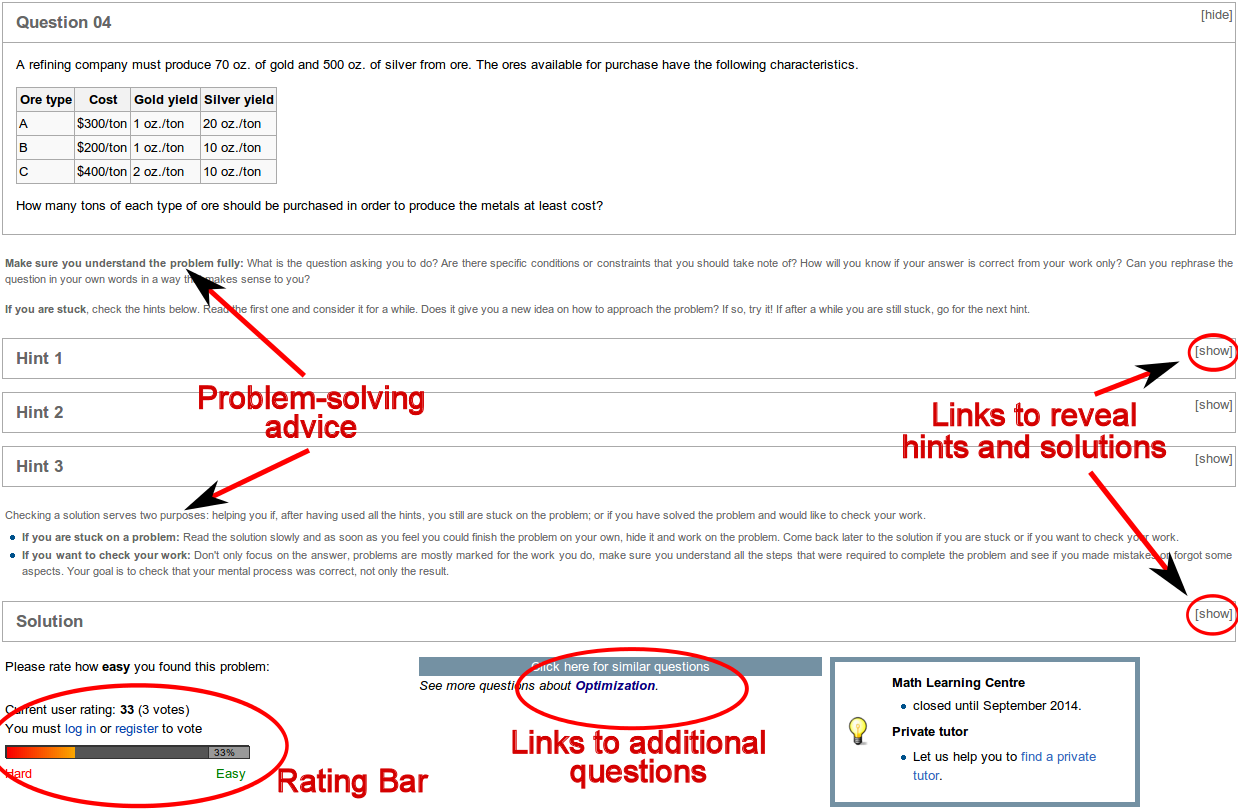
\includegraphics[width=\textwidth]{figs/Question_Page_annotated.png}
\caption{This graphic highlights several of the interactive features that students encounter on a question page.}\label{fig:question_page_annotate}
\end{figure}

\subsection{PEER REVIEW}\label{sec:Peer_Review}
One of the main advantages of the wiki system is the ability to collaboratively edit central documents.  For the MER, we built on this feature by implementing a dynamic peer review process. Unlike many static methods to disseminate mathematics questions and solutions, the MER wiki content can continually be updated and improved upon; questions and solutions pass through multiple quality-filtering processes.  First, there is an initial content creation phase where wiki contributors design hints and detailed solutions for an exam question.   Once a wiki contributor has transcribed a question, or written a hint or solution to a problem, the content is immediately accessible to everyone, but the content is labelled with a warning that there has been no review of the contribution.  Next, an open review process occurs, where the larger community of wiki contributors analyze the hints and solutions for two equally important attributes: correctness and value to the mathematical learning process.  Once solutions and the corresponding hints have met the wiki’s standard of excellence, it is finally flagged as a good quality solution and indicated as such to users who visit the corresponding question page.
\\\\
\noindent{}The review process described above was motivated by the long standing use in traditional print mediums such as academic journals but the added dimension of a wiki multimedia platform allows for greater control in maintaining quality as new issues arise.  These new issues can range from content correctness to logical or typesetting errors found in a reviewed solution. At any point in the review process, all wiki users and contributors are able to post comments on the content and suggest further improvements in the solution’s clarity or presentation, including after a solution has been deemed good quality.
\\\\
\noindent{}One such example of user-contributor interaction is shown in Figure \ref{fig:Comment_Question}.  A student is struggling with an integration concept and one of the contributors provides further explanation to the student using mathematical syntax.  If a solution that has been peer-reviewed and accepted but is found to have an error, it can be flagged as erroneous, allowing contributors to improve the solution and re-flag it for review.  This additional editing flexibility is important for many reasons.  First, an incorrect solution that was erroneously accepted by a peer can later be corrected.  An excellent example of this is in Figure \ref{fig:Comment_Error} where a question originally flagged as high quality has been found to have a mistake by one of the many users.  A contributor was able to reply to this user, make the necessary corrections to the solution and resubmit it to the queue for review.  This dynamic exchange noticeably improves on the paper exam solution packages which lacked quality control. Second, with a print model, it might not be economically viable to
correct a small calculation error. However, in an online resource where micro edits are easy, such corrections can occur quickly, cost nothing, and be available to users instantly after the update occurs.
\\\\
\noindent{}Even when a solution is correct technically, a student may comment that a solution approved as good quality is in fact difficult to comprehend, bring it to the attention of the contributors who can then improve on the clarity of the solution.  This can be particularly useful if the techniques covered in class are different than those of the current solution, if the notation is unfamiliar to the students, or if a mathematical step needs further clarification.  Figure \ref{fig:Comment_Suggestion} demonstrates a user asking for clarification on an alternative technique to solving a problem.  A contributor then provides new insight for the student but ultimately creates an entirely new, alternative solution for the problem.  Improvement could come from a contributor's perspective where they think of an alternative hint or solution, which they can then add and flag for review.
\begin{figure}[H]
\centering
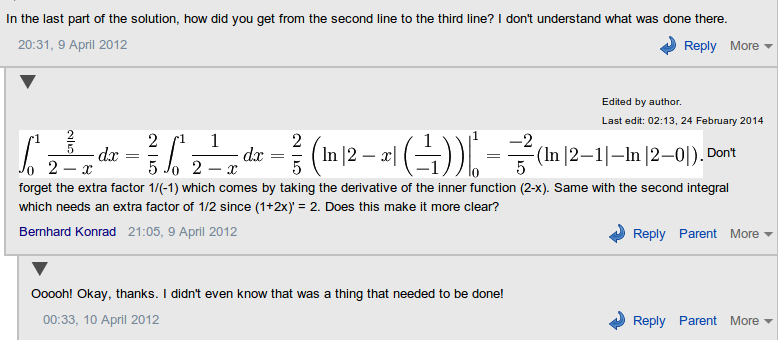
\includegraphics[width=\textwidth]{figs/Comment_Question.png}
\caption{A student uses the discussion forum to ask wiki contributors to clarify the solution presented.  After a brief discussion, the matter is resolved.}\label{fig:Comment_Question}
\end{figure}
\begin{figure}[H]
\centering
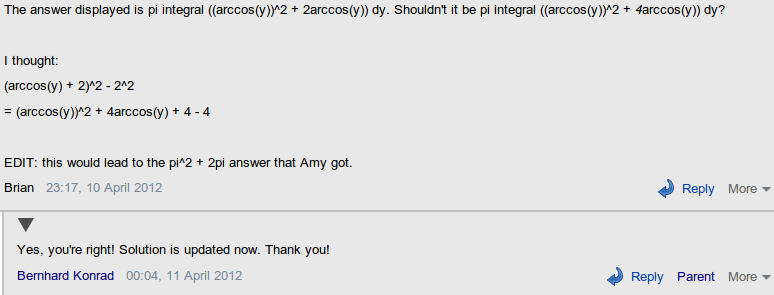
\includegraphics[width=\textwidth]{figs/Comment_Error.png}
\caption{A student finds an error in the solution and addresses it on the discussion page.  Wiki contributors verify the mistake and make the appropriate corrections.}\label{fig:Comment_Error}
\end{figure}
\begin{figure}[H]
\centering
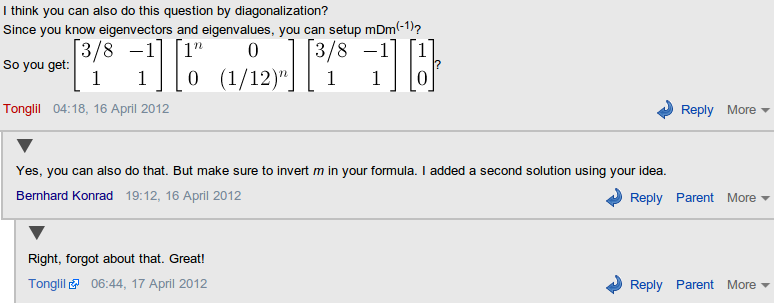
\includegraphics[width=\textwidth]{figs/Comment_Suggestion.png}
\caption{A student finds an alternative approach to solving the problem and suggests the solution on the discussion pages.  A contributor acknowledges the alternative technique and creates a new secondary solution based on the student feedback.}\label{fig:Comment_Suggestion}
\end{figure}

\subsection{STUDENT FEEDBACK}\label{sec:Student_Feedback}
MediaWiki has the built-in option to comment on pages, meaning any user can comment on question pages in order to ask for help or make suggestions.  However, we noticed that the option was not being fully utilized on our wiki. This might be because commenting required a UBC-specific login that may breach the student’s anonymity. To encourage more interaction we embedded a link to a form where students can anonymously ask questions or report typos. Since this addition, significantly more errors have been pointed out and quickly fixed, and solutions were also clarified at a much higher rate. Once a student comments on a solution, a contributor can fix the error and resubmit the question to the peer review process to ensure high quality and no newly introduced typos (see Figures \ref{fig:Comment_Error}, \ref{fig:Comment_Question}, and \ref{fig:Comment_Suggestion}).

\subsection{TAGGING SYSTEM AND TOPICS PAGES}\label{sec:Tagging_System}
The tagging system on the wiki is analogous to the topic index found at the back of many textbooks. Each question is categorized based on a list of topics that we create, adapt and modify as we see fit.  Once a question is entered with hints and solutions, a tag is attached to the problem to identify the mathematical concept it belongs to. At the time of this writing, we have over 150 different tags ranging from \textit{affine cryptosystems} to \textit{work} (Figure \ref{fig:wiki_tags}). This system is a key feature that helped propel the wiki from an exam database to an educational resource. Examination questions do not necessarily follow the same logical order that an instructor would choose to teach their course. Thus, for the wiki to be of use year-round we needed this tagging system to help organize questions by topic. Each tag has its own wiki page where all questions of this tag are listed and organized both by course and in bulk. 

\begin{figure}[H]
\centering
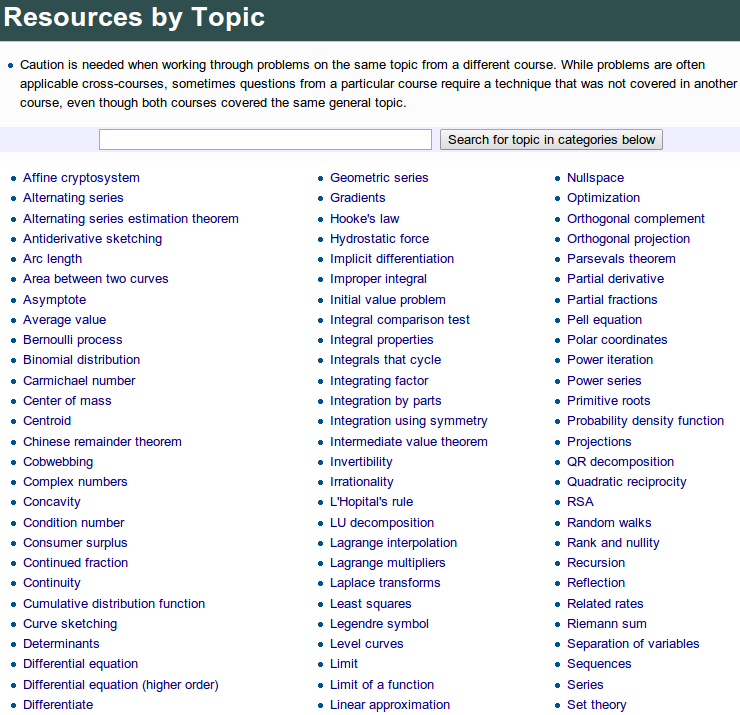
\includegraphics[width=\textwidth]{figs/Tag_List.png}
\caption{A list of topics available for study on the MER wiki up-to-date as of the writing of this paper.}\label{fig:wiki_tags}
\end{figure}

\noindent{}Being a dynamic medium, the functionality of these category page goes beyond a standard index. In particular, we have added videos on the topics pages. Videos included here range from giving concrete examples to discussing the underlying concepts in more detail, both of which help to promote student understanding. The majority of these current videos were created by Patrick Jones\footnote{see \url{http://patrickjmt.com/}} and are hosted on YouTube. We also include videos from local instructors as well and hope to continue to expand our database. The wiki can embed these videos directly on the tagging pages and thus students can not only use the topic page to locate similar problems on these pages, but can also learn from videos relevant to the concept on the tagging page.  A sample tag page can be found at \url{http://wiki.ubc.ca/Category:MER_Tag_Fundamental_theorem_of_calculus} (see Figure \ref{fig:topic_page}.

\begin{figure}[H]
\centering
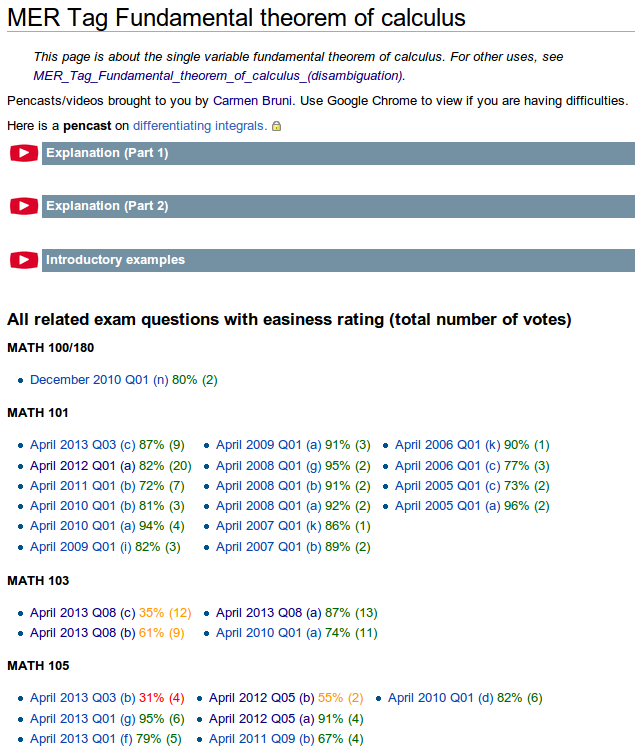
\includegraphics[width=\textwidth]{figs/Topics_Page.png}
\caption{An example of a topic page that students would access from the list in Figure \ref{fig:wiki_tags}.}\label{fig:topic_page}
\end{figure}

\noindent{}With the promotion of topics pages, the wiki saw a much heavier use during the entire term, not only around final exam period (see Section \ref{sec:Usage_Data} on the usage statistics). Students can easily obtain access to a hand-picked selection of videos and to relevant final exam problems that can help them study for midterm test and to reinforce concepts taught in class. This is also a resource that instructors can easily direct their students toward which can be used to help get additional support in mathematics courses. For example, in a lecture of a class taught by Carmen Bruni, a student asked for another example of an “integration by parts” problem. Instead of having to design an example in class or taking one from the textbook, the instructor was able to go to the corresponding topic page on the wiki to select a relevant problem of suitable difficulty, and get his students to complete it in class. The instructor offered hints in two minute intervals and finally revealed the step by step solution for students to verify their work.  In another example, Iain Moyles was teaching a second year course that relied heavily on first year prerequisite courses currently featured on the MER wiki.  When students struggled with topics from those courses, the instructor was able to direct them to various tagging pages on the wiki, eliminating the need to review prerequisite topics in class and giving the instructor the opportunity to introduce students to a free, easy-to-access, and relevant resource for their personal review.

\subsection{RATING BAR}\label{sec:Rating_Bar}
One of the more fun and social interactive aspects of the wiki is the ability for students to vote on the easiness of a question. Students can rank how easy they perceive a problem based on a 0-100 point scale. In order to vote on the difficulty of a question, users must be logged into the system with their UBC account, which allows users to update their vote and prevents multiple votes from the same person, see Figure \ref{fig:Rating_bar}). Unlike the discussion page commenting previously mentioned, the rating of an individual user is not public even with logging in.  At the time of writing, over 700 questions have received a total of over 3000 ratings The average rating is displayed on every question page so that students can see how challenging their peers perceive a problem before they start their own solution attempt.

\begin{figure}[H]
\centering
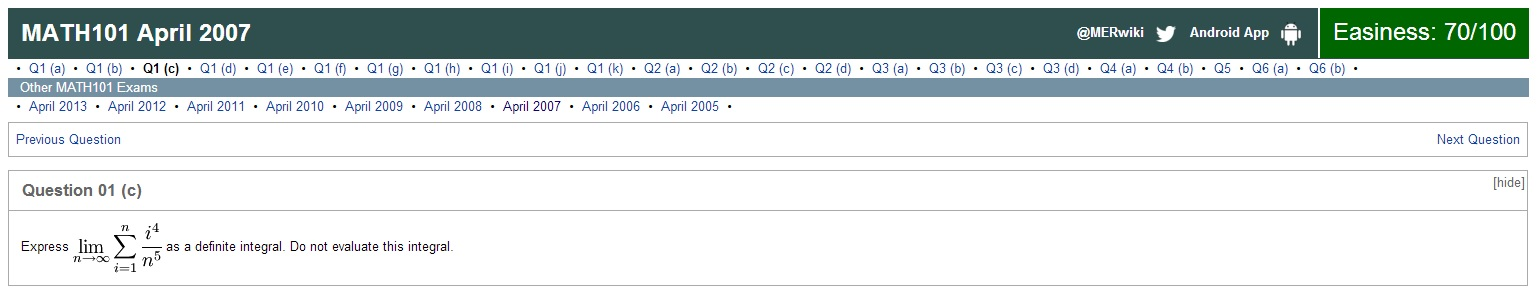
\includegraphics[width=\textwidth]{figs/easiness_rating.jpg}
\caption{The rating for a question is shown in the top right-hand corner of a question.  The value is displayed in a colour gradient from green to red with green representing very easy problems and red representing very difficult problems.}\label{fig:Rating_bar}
\end{figure}

\noindent{}The average easiness rating of each question is also displayed in the list of questions on the topic pages (Figure \ref{fig:wiki_tags}). This allows users to personalize and focus their learning even more by choosing questions at an appropriate difficulty level in a particular topic.  After completing the questions, students can compare their mastery of the material to the listed score and reassess their study directions based on where their personal rating measures in relation to the group.

\subsection{INTERACTIVE SYLLABUS}\label{sec:Interactive_Syllabus}
One of the authors of this paper, Carmen Bruni, developed a syllabus for Math 103\footnote{see \url{https://github.com/cbruni/MATH-103-Syllabus-UBC-}}, an integral calculus course for life science students offered at UBC. It was unique in that the document contained learning goals intertwined with sample problems to reinforce the learning objectives and these problems came with a solutions guide. Additionally, at the end of each section, there was a link to the wiki topic pages where students could see the aforementioned videos and question pages on the topics covered in the relevant chapter of the course. 
This innovative classroom feature was then extended to the wiki with the inclusion of a dynamic syllabus.  We have placed the course objectives directly on the wiki (Figure \ref{fig:Syllabus_Math103}) instead of just in a downloadable pdf document.

\begin{figure}[H]
\centering
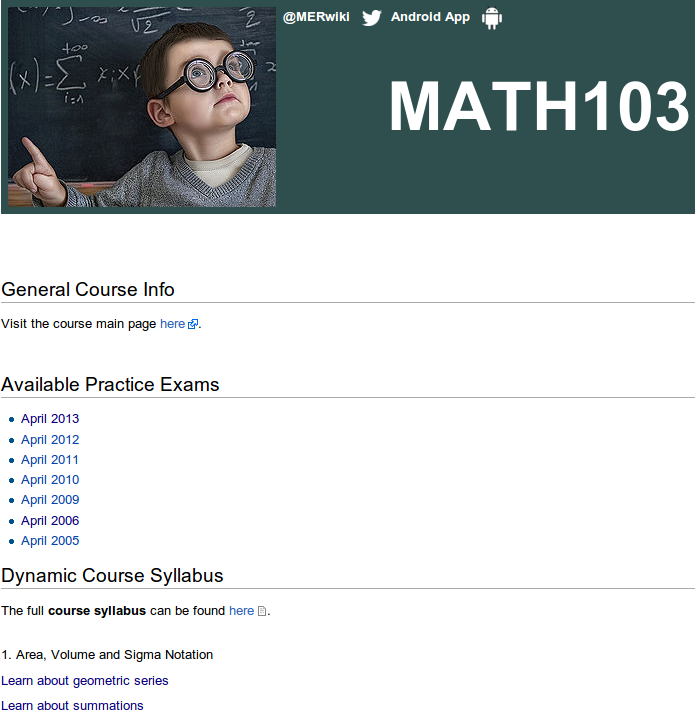
\includegraphics[width=\textwidth]{figs/Syllabus_Math103.png}
\caption{The course syllabus allows topics presented in class to be directly linked to topics on the MER wiki.  In this particular example we see information for the Math 103 class at the University of British Columbia.}\label{fig:Syllabus_Math103}
\end{figure}

\noindent{}Instructors can direct their students to the relevant sections on a midterm exam so that students can go to the wiki at their own leisure and have access to a plethora of sample problems over a number of years, exams and courses. Now students have well written sample problems with solutions coming from previous examinations and they have hints to guide them through the steps of the solution-finding process. This is in contrast to the typical approach, whereby students are given either midterm solutions that often contain little beyond the final answer or textbook questions to solve which often do not accurately reflect the difficulty of midterm and final exam questions.

\subsection{STUDENT CONTRIBUTIONS AND SUSTAINABILITY}\label{sec:Student_Contributions_and_Sustainability}
One of the most challenging aspects of a large volunteer-coordinated open project is that working hours are limited.  Furthermore, since the workforce consists primarily of graduate students, we are restricted by our degree completion timelines.  In an effort to alleviate some of these constraints, we are seeking means with which we could transfer the creation process to the same community that uses the service, that is, turn the user into a contributor.  One obvious attempt might be to open the wiki for editing by the public, in the way that Wikipedia and other public wikis are.  However, in our situation, as university mathematics is a specialized field, we have concerns about the pedagogical standard in the presentation of hints and solutions, not to mention technical challenges like using the typesetting software LaTeX.  Thus, when it came to sustainability, we sought other pathways, in particular, facilitating contributions from undergraduate student users.  We describe below two strategies we recently implemented to increase student contributions and therefore long-term project sustainability.
\\\\
\noindent{}During the 2014 April exam period, we held a solution writing contest for undergraduate students. The students could propose solutions to exam problems that were not yet on the wiki and submit them via an online form.  These solutions entered our usual peer-review process and eventually became part of the wiki.  The aim of this contest was to reduce the workload of content generation and free up time for editing and polishing work to improve its overall quality. Students could submit as many solutions as they wanted and every solution that was well written resulted in a ballot for the authoring student.  At the end of the contest we had 22 submitted solutions and we selected three ballots at random to win gift certificates to food services on campus. We advertised the winners on the MER wiki to demonstrate that the contest had real prizes and hopefully generate an even stronger interest in future iterations of the contest. In addition to alleviating the workload on contributors, this contest generated interest from students on continuing their work as some students inquired about a more permanent role in creating solutions.
\\\\
\noindent{}Another approach was implemented by Iain Moyles when he was teaching a third year course on linear algebra.  Realising the importance of being able to converse about mathematical concepts with peers, he devoted 10\% of the course grade to a math communication project.  To obtain this grade, students had to write solutions to previous exams for the course, in a similar style to exam solutions published on the MER wiki. Thus students were transformed from users to wiki contributors.  They were expected to independently work on their solutions at any point through the term.  To ensure a high solution quality, a second portion of the grade was to critique the solutions of their peers in a way similar to our peer-review system used in the wiki.  The class had 110 students enrolled and this lead to a generation of over 300 solutions.  The MER wiki itself uses LaTeX which is a hurdle for users new to typing mathematics not to mention the additional overhead of creating question pages and managing review flags. To alleviate this barrier a third party forum site was chosen to facilitate the logistics of entering their solutions was easier for students. The forum offers a generous LaTeX toolbar that facilitates entering solutions and an organizational scheme that makes it easy to tell when other students have reviewed problems. Course surveys at the end of term showed this idea was well received as students remarked they were essentially getting grades to study and that many would have done the old exam questions anyway in a preparation for their final exam.  Many also remarked that having to develop solutions from an instructional perspective led to a deeper understanding of the course material.  This idea has great potential; by splitting the workload over a large number of people, we were able to increase our total content by about 25\% in a time period of only two months.

\section{USAGE DATA}\label{sec:Usage_Data}
To measure usage of the UBC wiki, user data is collected via Google Analytics. We have analyzed the MER wiki specific data to gain insight into when, how, and how much students use our resource over the duration of their course. In this section we display the available data and mention how it could be used to understand how students approach math problems in general and how they prepare for final exams in particular.

\begin{figure}[H]
\centering
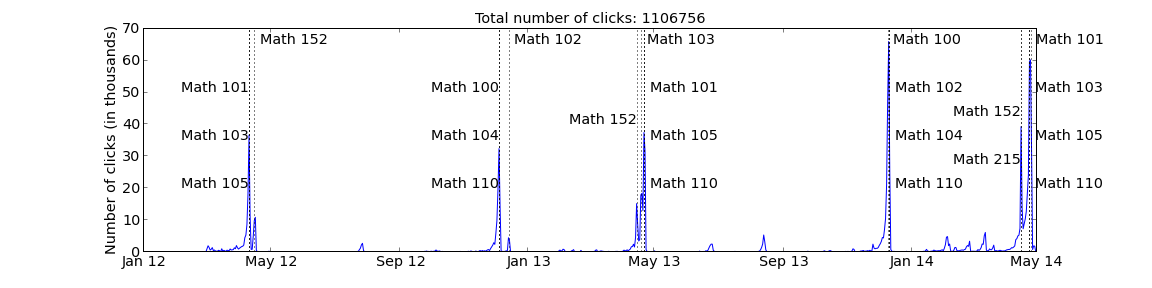
\includegraphics[width=\textwidth]{figs/total_number_of_clicks_time_series.png}
\caption{This shows the total amount of times users clicked something on the MER wiki as a function of time.  The exams during the fall and winter terms are also overlay.  There is a strong agreement between exam times and wiki usage.  Small spikes throughout the year correspond to the summer exam period or midterm examinations.}\label{fig:total_number_of_clicks_time_series}
\end{figure}

\noindent{}Figure \ref{fig:total_number_of_clicks_time_series} shows the total number of times any MER wiki page was accessed (single page request, or click) since its inception on February 20th 2012. Comparing the corresponding terms from 2012, 2013 and 2014, we see a steady increase in the overall wiki use. This is most likely due to a combination of several factors, mainly an increase in the number of available questions, word of mouth as previous users recommend the resource to new students, and improved marketing. Overlying the dates of the final exam, we quickly identify the usage building up to and peaking just before the final exam. Note, however, that the more recent term also show several small peaks around the time of the midterms, a result of our initiative towards transforming the wiki to a general educational resource by adding features such as dynamic syllabi and topic pages.

\begin{figure}[H]
\centering
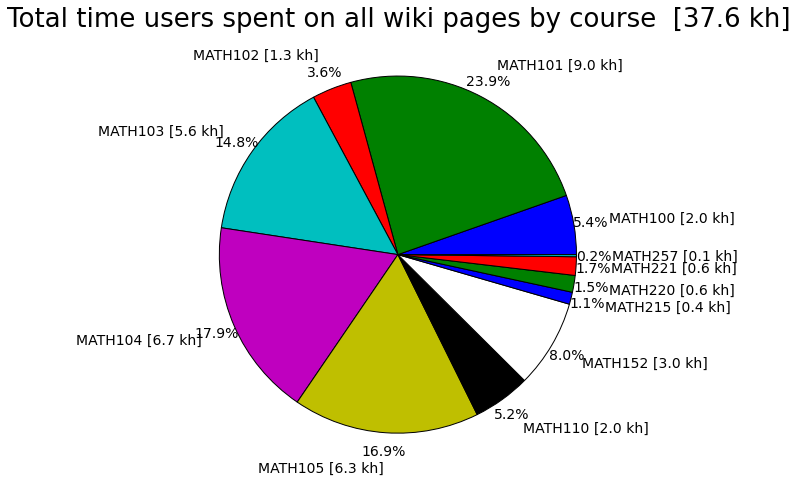
\includegraphics[width=\textwidth]{figs/total_time_per_course.png}
\caption{This shows the fraction of total viewing time separated by course.  The total viewing hours at the time of writing is approximately 37.6 thousand.}\label{fig:total_time_per_course}
\end{figure}

\noindent{}Figure \ref{fig:total_time_per_course} shows how much total time students have spent on each course since the inception of the wiki, which add to a total of approximately 37.6 thousand hours at the time of writing. It highlights our focus on first year math courses which, at the time of this writing, have 36 complete exams, compared to the 11 currently available for courses at second year level or higher.  One of the motivations for this focus is the high enrollment in first year classes (approximation 5000 students) compared to the more specialized upper division courses that service a smaller portion of the student population.  Further, it is more likely that a first year student will be unfamiliar with the problem solving strategies and logical skills involved with many of the problems and we want to focus on enhancing that ability.

\begin{figure}[H]
\centering
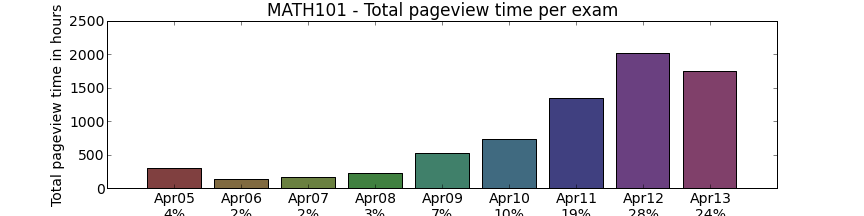
\includegraphics[width=\textwidth]{figs/total_pageview_per_exam_101.png}
\caption{This shows all the exam viewings for a single course Math 101 at the University of British Columbia.}\label{fig:total_pageview_per_exam_101}
\end{figure}

\noindent{}To understand how students use the wiki we plot the total time spent per exam, cummulatively on all corresponding question pages. Figure \ref{fig:total_pageview_per_exam_101} shows this data for Math 101. Note that the April 2013 exam was not available until early 2014. It shows that students use the most recent exams when preparing for their finals.  While historically, the core concepts for each course have remained relatively static, using the most recent exams is likely a reflection of the students’ expectations that the testing style is most relevant with exams chronologically closer to their own.

\begin{figure}[H]
\centering
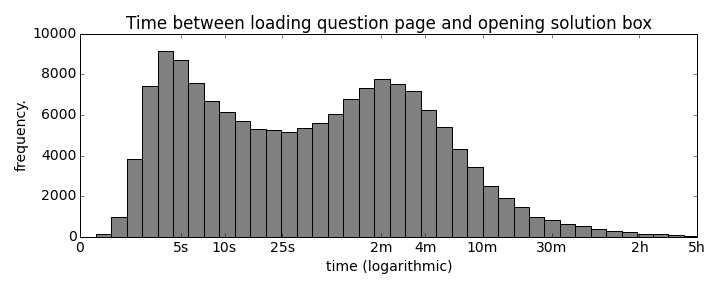
\includegraphics[width=\textwidth]{figs/2013_Term2_delta_t.png}
\caption{This shows the time differential between when a student enters a question page anywhere on the MER wiki and when they click the solution.  This data is for the exam period of April 2014 only.}\label{fig:2013_Term2_delta_t}
\end{figure}

\noindent{}When a question page is loaded the solution box is initially closed. In order to see if students solve questions one-by-one on their computer, we plot the delay between page load and opening of the solution box in Figure \ref{fig:2013_Term2_delta_t}. Noting the logarithmic x-axis we observe two humps in this time delay, the first around a few seconds, the second around a few minutes. This data may suggest that a large group of students do not solve the exam questions inependently, but rather work through the given solutions. At the same time, it is not uncommon to see students spend several minutes with the problem and hints before checking the solution, which may indicate that a large group of students do work through the problems one-by-one on their computer.

\begin{figure}[H]
\centering
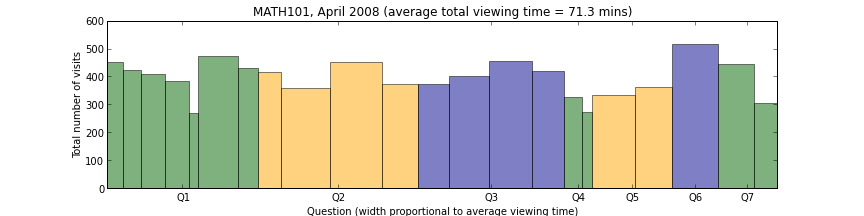
\includegraphics[width=\textwidth]{figs/question_dist_MATH101April_2008.png}
\caption{This is a question breakdown for the April 2008 Math 101 exam at the University of British Columbia.  The height of the bars indicate the number of times the question was viewd while the width of the bars indicates the average time spend on that particular question.  The colour coding indicates that the question had multiple parts.}\label{fig:question_dist_MATH101April_2008}
\end{figure}

Figure \ref{fig:question_dist_MATH101April_2008} shows the average time total number of visits of each question page for the Math 101 April 2008 exam.  The motivation for this statistic is that, we expect students will keep a page open while they’re working on a problem.  Therefore, it is reasonable to infer that questions with large times could be difficult to solve or are unclear.  In the figure, Question 1 is a short-answer question, where each part is worth the same number of points. Question 1(f)\footnote{see \url{http://wiki.ubc.ca/Science:Math_Exam_Resources/Courses/MATH101/April_2008/Question_1_(f)}} stands out as a short-answer question where students spend most of their time. In fact, it takes students about as long to complete this question as the longer question 6. This may or may not have been intended by the composer of the exam, but having a wiki that tracks usage data allows instructors to automatically gather this kind of information.  This could allow future instructors to decide on a reasonable question length and analyze which questions are suitable for the exam time allotted for short-answer questions. The other questions that stand out in this graph for receiving a very low average time are Q1(e) (probability) and Question 4 (higher order differential equations), which are both on topics that have been removed from the course curriculum as of 2009.

\section{CONCLUSIONS}\label{sec:Conclusions}
Throughout its history, the MER wiki has been evolving from a static exam review resource to a dynamic content collection with significant potential for future improvements and growth.  We have created an online resource where students can study math via worked examples, watch related videos and impact the available content directly through their feedback. Students come to the wiki with a basic theoretical knowledge/background and are then able to work through problems, guided by hints and thorough solutions, an interactive syllabus for their course, videos, and the easiness ratings of their fellow students.  In addition, they can submit questions and suggestions about the content and rate problems themselves.
\\\\  
\noindent{}This history of continual growth and improvement means we are always asking ourselves “what next?”  The following list describes some goals and visions that are in progress or that our team is considering for the future:
\begin{itemize}  
\item \textbf{Impact study:} We received funding to develop and implement an academic study of how students use the wiki and its effectiveness as a learning tool.  That study is well underway, and we are looking forward to analyzing results and using the conclusions in order to further drive development of our resource.
\item \textbf{Personalization:} Automatically generate smart personalized learning plans for students through an external app. Students using this type of feature could receive specific recommendations of problems to try, make problem lists, track their progress, and much more.
\item \textbf{Data analysis:} From an instructor’s perspective, data relating to the ratings bar could radically change the way exams and even courses are designed. With these votes, we can get access to large quantities of data given freely to us by students describing the difficulty of exam questions. The data is also publicly available which is in stark contrast with exam data mining. While writing future exam questions, instructors can predict perceived difficulty by comparing it to a similar version currently on the MER wiki. If an entire subset of questions in a given topic appear to be extremely difficult, it could be an indicator that the course needs to be designed differently to better educate the students on the particular topic.
\item \textbf{Student-generated content:} We have already entered the initial phase of adding student-generated content to the wiki by allowing students to submit content via a web form and through the third year summer semester course on linear algebra described in Section \ref{sec:Student_Contributions_and_Sustainability}. We can then review the content and post it to the wiki. Ultimately, if we continue to pursue this we would want students to have direct access to place content on the wiki and eliminate the need for a transfer process. This would blur the definitions of user and contributor and create a more authentic community experience.
\item \textbf{Open textbook:}  As we continue to add features to our wiki our project is propelling towards an interactive open textbook experience. Most open textbook conversations revolve around creating a standard written textbook that is open access; the MER wiki is a multimedia learning pod which can teach students concepts through traditional text, but also through images, videos, forum discussions and of course worked solutions. This new dissemination model can really change the interactive experience a student has with an open textbook.
\end{itemize}
\noindent{}For all its potential, the future success and development of the MER wiki requires a paradigm shift as it develops a new math education culture of accessibility in alternative mediums. The MER wiki represents a significant deviation from traditional resources available to students outside of the classroom and some instructors, administrators and decision-makers may be reluctant to embrace these changes or participate in the new culture. In addition, despite research that shows its effectiveness as a learning tool, some may have reservations about posting worked problems, our primary content offering.  Through our previous discussions and observations of student comments, we feel strongly that the wiki structure with background material, hints, and solutions does help student learning and offers a lot of potential for improving the undergraduate math education experience.  We also believe that the marriage of content, technological innovation, and accessibility on the MER wiki represents one face of the future of education.  
This resource is constantly changing and evolving. Even as you read this paper, the wiki has likely changed, expanded and improved in usability and sustainability. It is this dynamic feature of the wiki that makes it a truly amazing project to be a part of and to watch develop into a widely used resource for undergraduate students. This group of authors cannot wait to see how the future of this resource can be used to shape new generations of mathematicians.

\section{ACKNOWLEDGEMENTS}\label{sec:Acknowledgements}
On title page.


\begin{thebibliography}{1}

\bibitem{CS2}
Graham~A. Cooper.
\newblock Effects of schema acquisition and rule automation on mathematical
  problem-solving transfer.
\newblock {\em Journal of educational psychology}, 79:pp. 347 -- 362, 1987.

\bibitem{PM}
Fred~GWC Paas and Jeroen~JG Van~Merri{\"e}nboer.
\newblock Variability of worked examples and transfer of geometrical
  problem-solving skills: A cognitive-load approach.
\newblock {\em Journal of educational psychology}, 86(1):122, 1994.

\bibitem{CS1}
John Sweller and Graham~A. Cooper.
\newblock The use of worked examples as a substitute for problem solving in
  learning algebra.
\newblock {\em Cognition and Instruction}, 2(1):pp. 59--89, 1985.

\end{thebibliography}

%\bibliographystyle{unsrt}
%\bibliography{bib}

\section*{APPENDICES}

\appendix

\section{WIKI IMPLEMENTATION}\label{sec:Appendix}

This appendix will briefly discuss the implementation of the MER wiki, with an emphasis on how we utilized particular aspects of the MediaWiki platform to meet our design needs.
\\\\  
\noindent{}One of the foundational design choices of the wiki was putting each question along with its associated hints and solutions on an individual Question page.  Question pages are grouped as subpages of their originating exam, and exams are grouped as subpages of their respective courses.  All course pages are linked to from the front page of the resource, which also displays a summary of the amount of available content for each course.
\\\\
\noindent{}MediaWiki’s template and transclusion functionality is the fundamental building block used to implement the design scheme described above.  Transclusion is a MediaWiki feature in which the content of a wiki page can be embedded in another page.  Templates are a special type of wiki pages meant for transclusion in other wiki pages, creating identically formatted pages whose source code is in one location.  We used templates to frame most pages on the MER wiki, most notably the individual question pages.  Implementing the question page as a template means that if we want to change the layout of the question pages, we need only edit the template and changes will be reflected on all the pages created with that template.
\\\\
\noindent{}The other primary MediaWiki feature used to construct the MER wiki is categories.  Categories are essentially tags that can be added to wiki pages; clicking on the tag will then list all pages with that tag.  We used category tagging in multiple ways on the wiki.  Categories facilitate our peer review process: each stage in the peer review process has a corresponding category, and  question pages are tagged with the appropriate categories to indicate their progress in the peer review process.  The topic tagging system of the wiki was also implemented using the categories feature.   Finally, we use categories as an organizational tool to keep track of our pages, templates and contributors.
\\\\  
\noindent{}Another advantage of the MediaWiki platform is the availability of free extensions that allow for the addition of extra features.  These include features as fundamental as the ability to render LaTeX in wiki pages to the advanced level of having a ratings bar for students to rate questions.  The DynamicPageList (DPL) extension has also been foundational in how we organize the MER wiki and present its content.  Other useful extensions we have used include: PageInCat, ParserFunctions, RightFunctions, Variables, Widgets and Category Tree.
\\\\  
\noindent{}In addition to focusing on student usability, we also built this resource with the requirements of efficient editing in mind, including an online peer review system and space for contributors to communicate and organize tasks.  For the latter, we created a separate set of wiki pages for administrator and contributor use.  These pages help us to keep track of which courses need to be updated as well as keep track of current open projects for the wiki. These pages include links to a contributor’s and developer’s manual which features a multiple-series how-to-contribute videos on youtube.  In addition, while most of our content related tasks (adding and editing solutions, creating new exams) are managed through these dedicated wiki pages for contributors, much of our development work has been organized through other online tools, notably Google Drive (for web forms and general documents) and a project management app named Hojoki that helps us to organize our tasks.  For more information on our design or implementation, please see our complete developer’s manual at \url{http://wiki.ubc.ca/Science:MER/Manual}.
\end{document}